\subsection{Workflows and Workloads}

The term ``workflow'' is used in many disciplines with different meaning. In the
field of scientific computing, ``workflow'' assumes different meanings depending
on the characteristics of the computation, of the software tools used to support
this computation, and of the resources on which it is performed. Further, a
workflow may indicate a whole application, a description of the computational
process of that application or, more commonly, a series of tasks related by data
dependences.

The lack of a consistent and shared definition of ``workflow'' hinders the
understanding of its properties and its relations with related concepts. For
example, we need to clarify the difference among ``workflow'', ``workload'',
``task'', or ``job'' but also between workflow ``template'' and ``instance'', or
``data-flow'' and ``control-flow''. This is precondition to specify properly the
design of software systems that support the execution of scientific
applications.

In this paper, we use the following definitions:

\begin{description}

  \item[Task.] A set of operations to be performed on a computing platform,
  alongside a description of the properties and dependences of those operations,
  and indications on how the dependences should be satisfied and the operations
  should be executed.

  \item[Job.] A unit of execution that performs one or more unit of work. Jobs
  relates to the resource on which they are executed. One or more tasks can be
  the units of work executed by a job.

  \item[Workload.] A set of tasks that can be executed concurrently, possibly
  related by a set of relations. For example, tasks of a workload can share one
  or more input files or communicate during execution.

  \item[Workflow.] Set of workloads, related by a set of relations that define
  the order in which each workload can be executed. Data dependences are the
  most common relations among workloads, used to define the precedence among
  their executions. Note that, formally, a workload can have a single task.

\end{description}

Each task may have an arbitrary number of properties like number of cores,
executables, or input/output files. Tasks may have precedence interrelations,
depending on their data dependences or any other type of dependency mandated
by the application algorithms. Tasks with precedence relations have to be
executed serially; otherwise, tasks can be executed concurrently. A workload is
defined as a set of tasks that can be executed concurrently. As such, a
workflow can be composed of a set of workloads.

The terms ``task'' and ``job'' are also used inconsistently across communities
that perform scientific computing. In this paper, ``job'' refers to the unit of
work that is submitted to a local resource management system (LRMS), like the
Slurm or PBS batch system of a cluster. As such, a task can become a job when
is scheduled on a resource that exposes a LRMS but can also become a virtual
machine or a container when bootstrapped on an infrastructure supporting
virtualization. Tasks can be statically or dynamically grouped into jobs,
depending on the resource capabilities and the task requirements.

Usually, workflows are represented as graphs in which tasks are vertices and
relations are edges~\cite{}. Often, graphs are supposed to be acyclic but graphs
with cycles have been used to represent workflows of workflows~\cite{}. In this
paper, a workflow template is a type of graph while a workflow instance is a
workflow template with specific vertices and edges. Further, a workflow instance
is ``abstract'' when no resource properties are available for all vertices,
``concrete'' otherwise~\cite{}. When not qualified, the term ``workflow''
indicates a abstract workflow instance.

\subsection{The ATLAS Monte Carlo Workflow}

The distinction between an abstract and concrete workflow instances highlights
an important element of the execution process of a workflow. Abstract workflows
can be interpreted as a formal description of the requirements for the workflow
execution, while concrete workflows can be interpreted as a formal description
of the workflow's execution process. The process of resource selection matches
the resource capabilities to the workflow requirements making possible the
transition from execution requirements to execution process.

Workload managers are those components of workflow systems or, more in general,
of distributed applications that enable resource selection, acquisition, and
use. The set of capabilities required by a workload manager mostly depends on
the heterogeneity and dynamicity of both the workflow and the resources.
Heterogeneity is a measure of the diversity of the workflow requirements and
resource capabilities that need to be matched to enable the execution of the
workflow's tasks; dynamicity is a measure of how much these requirements and
capabilities varies during execution.

The PanDA workload management system was initially designed to manage the
execution of static, relatively homogeneous tasks on dynamic but homogeneous
resources. Progressively, PanDA has evolved to enable the management of more
heterogeneous tasks and resources. In this paper we describe how the design and
architecture of PanDA has enabled executions of multi-threaded tasks on Titan,
currently the largest high performance computing (HPC) resource available in the
USA for scientific research.

Traditionally, the ATLAS workflow has been based on single-core tasks, executed
on Grid resources to process large amount (2TB) of input data divided into
discrete I/O units called ``events''. This approach has many merits: (i)
simplified process of resource selection under the assumption of homogeneous
resources and execution environments; (ii) opportunistic distribution of compute
tasks across resources based on contingent availability; (iii) relative
robustness due to the ability of re-executing failed tasks; and (iv)
multi-tiered distribution and storage of events' data.

Despite all the advantages, ATLAS workflows have evolved to include
compute-intense tasks that can benefit from multithreaded execution on HPC
machines. The Monte Carlo workflow~\cite{} is one of the largest workflows
executed by the ATLAS experiment and at least one of its stages can benefit from
large amount of parallelism. The Geant4 toolkit is used to simulate the passage
of particles through matter and\ldots

\begin{figure}
  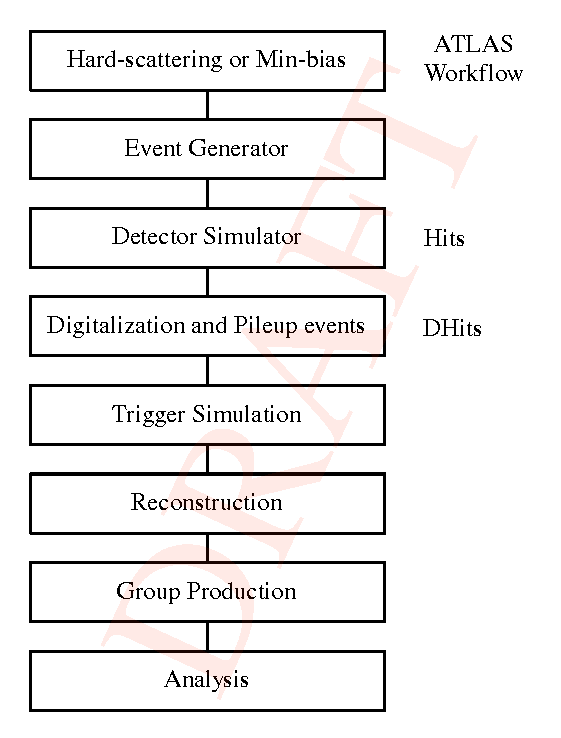
\includegraphics[width=\columnwidth]{figures/atlas_workflow.pdf}
  \caption{ATLAS Monte Carlo workflow.}
\label{fig:atlas_workflow}
\end{figure}
